\documentclass[12pt]{article}
\usepackage{settings}

\title{Interactive maps as a tool for visualising accessibility}
\author{Eemil Haapanen}

\begin{document}
\maketitle

\section{Introduction}
% What accessibility?
The term accessibility is central to this thesis.
In its most general sense, the word simply means how easy something is to access,
with all further meaning derived from the context in which the word is used.
This context could be 

% Geographical accessibility as a phenomenon in general, hard to measure
The general starting point for many definitions accessibility, in the geographical sense, is
\enquote{potential of opportunities for interaction} \parencite{han1959}.
Depending on the factors thought to impact that potential,
accessibility can be defined and measured in many different ways \parencite{pap2016}.
Even if just considering travel distance or time as a measure of access,
when including all the different things accessibility can be measured in relation to,
the amount of combinations gets out of hand fast \parencite{lev2020}.
In addition, accessibility is inherently tied not only to location
but also time \parencite{jar2018},
meaning every place in every time has a level of access
in relation to every other place \parencite{lev2020}.
All this makes measuring accessibility in a wholistic way a complicated task.

% hard to visualise too
Similarily to defining or measuring it, visualising accessibility is complex.
Accessibility visualisations are often constrained to displaying access in relation to
a limited number of pre-selected places (for example \textcite{wei2018}),
or composing an accessibility index that can be calculated and mapped for all locations,
in relation to potentially many different things and locations (for example \textcite{kim2019}).
However, more complex accessibility measures tend to lead to
less usable presentations \parencite{te2014},
while mapping more simple measures could lead to an influx of variations to present.
For example separating different travel modes, times of day or target locations
would multiply the amount of visualisations needed to present accessibility.

% how interactivity benefits accessibility visualisation (because of how accesibility is)
Even if visualising every aspect of accessibility from everywhere to everywhere is impossible,
interactive visualisations could offer some benefits for presenting accessibility.
After all, a key principle of interactivity in map presentations is
the map user's ability to change the content of the map \parencite{rot2013}.
For visualising accessibility this could mean, for example,
interactive selection of location or travel mode instead of
a static accessibility index that, to a varying extent, tries to account for everything.
Scientific literature on the topic seems to support the idea of
interactivity in accessibility visualisation, even indicating a need for such presentations.
In a study focusing on the usablity of different accessibility instruments and visualisations,  % accessibility instrument
\textcite{te2014} highlight the importance of real-time interactivity between the map and the map user.
\textcite{but2018} state that for maps to efficiently communicate accessibility,
they should be as flexible and dynamic as possible.
However, \textcite{but2018} also note that these qualities are often missing in accessibility visualisations.
Along the same lines, \textcite{paj2021} find modern accessibility visualisations often complicated,
and lacking in interactivity and flexibility.

% research questions
% Communicating accessibility instead of analyzing it
% How to utilize interactive mapping in communicating accessibility
This thesis approaches accessibility from a cartographical angle,
especially in the context of interactive mapping.
There are three main research questions.
Firstly, how should accessibility be presented cartographically?
To answer this, I will go into detail of what makes accessibility an unique phenomenon,
especially from a cartographical point of view,
and what requirements this places on visual representations of accessibility.
Secondly, what value do interactive visualisations hold in the context of accessibility?
Here I will focus on the general theory of cartography and especially cartographic interaction,
also previewing previous interactive maps and presentations relative to the topic.
Thirdly, how should an interactive accessibility presentation be implemented?
The goal here is to develop an interactive web-based presentation of the
Helsinki Region Travel Time Matrix \parencite{ten2020}.
In addition to the insights gained from the previous research questions,
I will utilize an iterative development process with interviews
to keep in touch with the map user's perspective.


\section{Background}

% Currently I see the first two research questions as a sort of a background study
% necessary to form a theoretical base
% for the implementation of the interactive matrix visualisation.
% This is why I have placed them in a background section.

\subsection{Cartography}
Should this be here?

\subsection{Accessibility in the context of cartography}
This section focuses on the first research question:

\begin{displayquote}
What makes accessibility an unique phenomenon,
especially from a cartographical point of view,
and what requirements this places on visual representations of accessibility.
\end{displayquote}

This will be a litearture review.

What are the "normal" (cartography-wise) phenomena, do they exist?

\subsection{Interactive maps and their potential in presenting accessibility}
% Interactivity in general
% The default medium for viewing maps and geographical has long been digital.  % TODO add ref
% However, more and more devices allow also for interaction \parencite{mei2019}
The second research question:

\begin{displayquote}
What value do interactive visualisations hold in the context of accessibility?
(General theory of cartography and especially cartographic interaction,
previous interactive maps and presentations relative to the topic.)
\end{displayquote}

Here I will be doing literatrure review as well,
especially relating to the theory of cartography and interactive maps.
Themes such as critical cartography
and the qualitative nature of maps should be found here too.
When previewing previous accessibility visualisations,
some kind of a systematic comparison of previous work
could be a way to form a synthesis here.

\section{Study design}
Describe the study design in more detail.

\section{Data and methods}

This section will focus on the matrix visualisation.

\subsection{Data - Helsinki Region Travel Time Matrix}

General description of the matrix goes here.

\subsection{Methods}

I see the methods necessary to implement the visualisation belonging to two themes:
Methods for figuring out how the map should be
and methods for actually making the map be that way.

For figuring out what the map should be like,
I have (hopefully) at this point already formed some ideas from the background section.
To complement those, and to keep the qualitative aspect of cartography relevant,
interview(s) will be used alongside the development process.

From the technical angle, there are three main components to the map:

\begin{enumerate}
	\item Preprocessing of the matrix to a mappable format
	\item A back-end to serve the matrix
	\item The web map application
\end{enumerate}

See figure \ref{fig:architechture} for my idea of what the architechture might look like.

\begin{figure}[H]
	\centering
	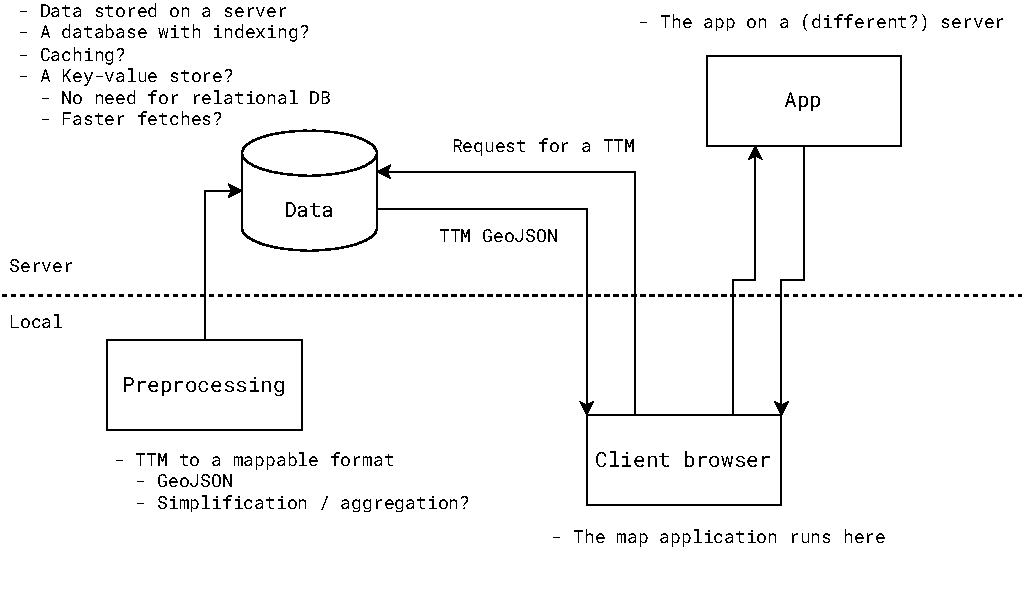
\includegraphics[width=1\textwidth]{images/architechture}
	\caption{Architechture}
	\label{fig:architechture}
\end{figure}

When developing the visualisation, the priority should be on the map application.
However, the development must progress on all components as an iterative process,
where producing a minimal working state should be the first goal.
Something that, to some extent, works, makes discussion about the map possible,
which in turn should keep development progressing towards the right direction.

It should also be noted that the number of techical options for implementing the map is large.
Questions such as which mapping library or UI framework to use,
or how to preprocess the matrix data should be covered here too.
Depending on the need and extent of comparisons between different technologies,
some synthesis could be formed about that too.

\section{Results}

Every research question should have some kind of a result to it.
The first two questions, being more focused on theory rather than implementation,
have their results already in the backround section,
since they are necessary for the rest of the thesis to make sense.
Still, some kind of a synthesis of those results should be here as well.

The results of the implementation of the matrix are, firstly, the visualisation itself,
but also the output of the interviews
and possibly of the technical comparison between technologies.

\section{Discussion}

Discussion and conclusions about the results

\section{Timetable}

I think the work needed to complete this thesis can be divided into three main themes:

\begin{enumerate}
	\item Background study / literature review to gain a theoretical base
	\item Comparing and learning technologies to gain a technical base
	\item The iterative development of the visualisation
\end{enumerate}

My planned timing for the thesis will be from now (summer) to the end of the year (winter).
Even though the themes above will overlap,
my goal is to focus on the first theme first (summer, early fall),
and after that progress towards the last theme (fall, winter).
Realistically, techonogical experimentation will be happening continuously,
but most likely more at the start.

\printbibliography

\end{document}